%%%%%%%%%%%%%%%%%%%%%%%%%%%%%%%%%%%%%%%%%%%%%%%%%%%%%%%%%%%%%%%%%%%%%%%%%%%%%%%
% CHAPTER 2: Literature Review
%       DUE: May 1, 2025
%     PAGES: 20-30
%%%%%%%%%%%%%%%%%%%%%%%%%%%%%%%%%%%%%%%%%%%%%%%%%%%%%%%%%%%%%%%%%%%%%%%%%%%%%%%
\chapter{Literature Review}
\label{chap:litreview}

\section{Introduction}
The landscape of Artificial Intelligence (AI)\index{Artificial Intelligence (AI)}, particularly Natural Language Processing (NLP)\index{Natural Language Processing (NLP)}, was significantly reshaped by the groundbreaking work conducted at Google Brain, documented in the seminal paper \textit{Attention Is All You Need} \parencite{RefWorks:RefID:81-vaswani2017attention}. This paper introduced the Transformer architecture\index{Transformer Model}, which leverages self-attention mechanisms\index{Attention Mechanism!self-attention} and serves as the foundation for modern Large Language Models (LLMs)\index{Large Language Models (LLMs)}. These models have demonstrated remarkable capabilities across a wide range of tasks, including text generation, summarization, translation, and question answering, often producing outputs nearly indistinguishable from human writing \parencite{RefWorks:RefID:89-badshah2024quantifying,RefWorks:RefID:35-verma2024journey}.

Despite these advancements, LLMs possess an inherent architectural limitation: a finite context window\index{Large Language Models (LLMs)!context window}. This window represents the maximum amount of text, measured in tokens\index{Tokens}, that a model can process simultaneously when generating a response or performing an analysis. Consequently, if critical information or dependencies within a document fall outside this fixed window, separated by a larger span of intervening text, the LLM may fail to capture the relationship or address the query accurately \parencite{RefWorks:RefID:100-kaplan2020scaling}. This limitation poses a significant challenge when analyzing large or complex documents where understanding relies on synthesizing information across distant sections.

A promising approach to mitigate this limitation involves transforming large, unstructured documents into structured representations using Knowledge Graphs (KGs)\index{Knowledge Graphs}. Through the extraction of key entities, relationships, and attributes from text and mapping them into a graph structure, it becomes possible to represent the document's core semantic content in a format amenable to computational analysis \parencite{RefWorks:RefID:102-hogan2021knowledge}. Such a structure allows for querying and reasoning over the entire document's scope, independent of an LLM's context window constraints, potentially enabling a more focused and comprehensive analysis for tasks like ensuring information integrity.

This chapter reviews the pertinent literature underpinning this approach, beginning with an examination of the development and characteristics of Large Language Models. It focuses on their capabilities and limitations, particularly the context window constraint. Subsequently, the text delves into the principles, construction, and application of KGs as structured knowledge representations. Key techniques for populating KGs from text via Information Extraction (IE)\index{Information Extraction (IE)} are then discussed, followed by an exploration of the challenges associated with processing large and complex documents, especially within the legal domain. The chapter concludes by defining the critical concepts of consistency\index{Consistency}, completeness\index{Completeness}, and coherence\index{Coherence}, surveying related work, and presenting a summary that motivates the proposed research direction.

\section{Large Language Models}
The trajectory of modern NLP took a significant turn in 2017 with the publication of \textit{Attention Is All You Need} by Vaswani et al. \parencite{RefWorks:RefID:81-vaswani2017attention}. This work introduced the Transformer architecture, which relies on self-attention mechanisms to weigh the importance of different words (tokens) in an input sequence. This design enables superior handling of long-range dependencies\index{Transformer Model!long-range dependencies} compared to previous dominant recurrent or convolutional architectures, thereby addressing critical bottlenecks in earlier sequence models \parencite{RefWorks:RefID:90-turner2024introduction,RefWorks:RefID:101-zhao2023survey}. This innovation paved the way for the development of increasingly powerful language models, such as Google's BERT\index{Large Language Models (LLMs)!BERT}, which introduced bidirectional pre-training \parencite{RefWorks:RefID:167-gardazi2025bert}, and OpenAI's influential Generative Pre-trained Transformer (GPT) series\index{Large Language Models (LLMs)!GPT} \parencite{RefWorks:RefID:92-gao2023examining}.

While research groups at numerous institutions continuously pursued improvements, the public release of OpenAI's \textit{ChatGPT}\index{Large Language Models (LLMs)!ChatGPT} on November 30, 2022, marked a pivotal moment. The event dramatically increased public awareness and accelerated the deployment of advanced conversational AI systems. It also catalyzed the development of competing models from major research labs, including Google's \textit{Gemini}\index{Large Language Models (LLMs)!Gemini} family, Anthropic's safety-focused \textit{Claude}\index{Large Language Models (LLMs)!Claude} series, and Meta's open-source \textit{Llama}\index{Large Language Models (LLMs)!Llama} family \parencite{RefWorks:RefID:93-team2024gemini,RefWorks:RefID:94-caruccio2024claude,RefWorks:RefID:95-grattafiori2024llama}. The proliferation of models is evident on platforms like Hugging Face\index{Hugging Face}, a central repository for AI models and datasets, which reportedly surpassed one million hosted models by late 2024 \parencite{RefWorks:RefID:84-edwards2024exponential}.

Functionally, LLMs process input text (a "prompt"\index{Prompt Engineering}) by converting it into numerical representations called tokens, often using techniques like Byte Pair Encoding (BPE)\index{Tokens!Byte Pair Encoding (BPE)} or WordPiece\index{Tokens!WordPiece} \parencite{RefWorks:RefID:103-schmidt2024tokenization}. The model then uses the complex patterns learned during pre-training on vast text corpora to predict subsequent tokens autoregressively\index{Large Language Models (LLMs)!autoregressive generation}, generating a coherent and contextually relevant output. Prompts can be engineered to elicit specific behaviors, including the analysis of substantial text provided for context (in-context learning)\index{Prompt Engineering!in-context learning}. For instance, an LLM can be prompted with a company's annual report to answer specific questions or to summarize key findings, tasks on which many current models perform reasonably well, provided the information falls within their processing limits \parencite{RefWorks:RefID:96-rzepka2023expert}. The architecture of the Transformer model is depicted in \cref{fig:transformer}.
\begin{figure}[H]
\centering
\begin{tikzpicture}[
    font=\sffamily,
    node distance=0.4cm,
    % Define styles for different types of nodes - with reduced widths
    block/.style={rectangle, draw, minimum width=2.8cm, minimum height=1cm, align=center},
    addnorm/.style={rectangle, draw, minimum width=2.8cm, minimum height=0.6cm, fill=gray!10},
    feedforward/.style={block, fill=blue!10},
    attention/.style={block, fill=orange!10},
    masked_attention/.style={attention},
    cross_attention/.style={attention, fill=purple!10},
    embedding/.style={block, fill=green!10, minimum height=1cm},
    softmax/.style={block, fill=red!10, minimum width=2.8cm},
    io/.style={ellipse, draw, fill=yellow!20, minimum width=2.8cm, align=center},
    plus/.style={circle, draw, inner sep=0pt, minimum size=0.4cm},
    connector/.style={-latex, thick},
    residual/.style={connector, gray},
    encoder_block_fit/.style={rectangle, draw, dashed, inner sep=0.4cm, label={[xshift=0.3cm, yshift=-0.4cm]above right:Encoder}},
    decoder_block_fit/.style={rectangle, draw, dashed, inner sep=0.4cm, label={[xshift=0.3cm, yshift=-0.4cm]above right:Decoder}}
]

%==============================================================================
% ENCODER SIDE (Left)
%==============================================================================

% Input nodes at the bottom
\node[io] (inputs) {Inputs};
\node[embedding, above=0.5cm of inputs] (input_embedding) {Input Embedding};
\node[plus, above=0.5cm of input_embedding] (pos_encoding_plus_in) {+};
% Repositioned label to the left to prevent overlap
\node[left=0.2cm of pos_encoding_plus_in, align=center, font=\small] (pos_encoding_in_label) {Positional\\Encoding};

% Encoder Stack
\node[attention, above=1.2cm of pos_encoding_plus_in] (enc_attention) {Multi-Head\\Attention};
\node[addnorm, above=0.4cm of enc_attention] (enc_addnorm1) {Add \& Norm};
\node[feedforward, above=0.4cm of enc_addnorm1] (enc_ff) {Feed Forward};
\node[addnorm, above=0.4cm of enc_ff] (enc_addnorm2) {Add \& Norm};

% Fit a box around the encoder stack
\node[encoder_block_fit, fit=(enc_attention) (enc_addnorm2)] (encoder_block) {};
\node[right=0.1cm of encoder_block, font=\Large] (enc_nx) {Nx};

%==============================================================================
% DECODER SIDE (Right)
%==============================================================================
\node[right=5.5cm of inputs] (outputs) [io] {Outputs \\ (shifted right)};
\node[embedding, above=0.5cm of outputs] (output_embedding) {Output Embedding};
\node[plus, above=0.5cm of output_embedding] (pos_encoding_plus_out) {+};
% Repositioned label to the right to prevent overlap
\node[right=0.2cm of pos_encoding_plus_out, align=center, font=\small] (pos_encoding_out_label) {Positional\\Encoding};

% Decoder Stack
\node[masked_attention, above=1.2cm of pos_encoding_plus_out] (dec_masked_attention) {Masked\\Multi-Head\\Attention};
\node[addnorm, above=0.4cm of dec_masked_attention] (dec_addnorm1) {Add \& Norm};
% Increased vertical spacing for Q line visibility
\node[cross_attention, above=0.8cm of dec_addnorm1] (dec_cross_attention) {Multi-Head\\Attention};
\node[addnorm, above=0.4cm of dec_cross_attention] (dec_addnorm2) {Add \& Norm};
\node[feedforward, above=0.4cm of dec_addnorm2] (dec_ff) {Feed Forward};
\node[addnorm, above=0.4cm of dec_ff] (dec_addnorm3) {Add \& Norm};

% Fit a box around the decoder stack
\node[decoder_block_fit, fit=(dec_masked_attention) (dec_addnorm3)] (decoder_block) {};
\node[right=0.1cm of decoder_block, font=\Large] (dec_nx) {Nx};

% Final output layers on top of decoder
\node[softmax, above=0.5cm of dec_addnorm3] (linear) {Linear};
\node[softmax, above=0.4cm of linear] (softmax) {Softmax};
\node[io, above=0.5cm of softmax] (output_probs) {Output\\Probabilities};

%==============================================================================
% CONNECTIONS
%==============================================================================

% --- Encoder Connections ---
\draw[connector] (inputs) -- (input_embedding);
\draw[connector] (input_embedding) -- (pos_encoding_plus_in);
\draw[connector] (pos_encoding_plus_in) -- (enc_attention);
\draw[connector] (enc_attention) -- (enc_addnorm1);
\draw[connector] (enc_addnorm1) -- (enc_ff);
\draw[connector] (enc_ff) -- (enc_addnorm2);

% --- Decoder Connections ---
\draw[connector] (outputs) -- (output_embedding);
\draw[connector] (output_embedding) -- (pos_encoding_plus_out);
\draw[connector] (pos_encoding_plus_out) -- (dec_masked_attention);
\draw[connector] (dec_masked_attention) -- (dec_addnorm1);
\draw[connector] (dec_cross_attention) -- (dec_addnorm2);
\draw[connector] (dec_addnorm2) -- (dec_ff);
\draw[connector] (dec_ff) -- (dec_addnorm3);
\draw[connector] (dec_addnorm3) -- (linear);
\draw[connector] (linear) -- (softmax);
\draw[connector] (softmax) -- (output_probs);

% --- Residual Connections ---
% Encoder
\draw[residual] (pos_encoding_plus_in.east) -| ++(1.7, 0) |- (enc_addnorm1.east);
\draw[residual] (enc_addnorm1.east) -| ++(0.5, 0) |- (enc_addnorm2.east);
% Decoder
\draw[residual] (pos_encoding_plus_out.west) -| ++(-1.7, 0) |- (dec_addnorm1.west);
\draw[residual] (dec_addnorm1.west) -| ++(-0.5, 0) |- (dec_addnorm2.west);
\draw[residual] (dec_addnorm2.west) -| ++(-0.5, 0) |- (dec_addnorm3.west);

% --- Encoder-to-Decoder Connections (Key/Value and Query) ---
% Red K,V line with more horizontal space to prevent overlap
\draw[connector, thick, red] (enc_addnorm2.east) -- ++(1.5, 0) |- node[pos=0.70, below, font=\tiny] {K} node[pos=0.75, below, font=\tiny] {V} (dec_cross_attention.west);

% Blue Q line is now a clean vertical path
\draw[connector, thick, blue] (dec_addnorm1.north) -- node[pos=0.5, right, font=\tiny] {Q} (dec_cross_attention.south);

% *** MODIFIED NODE FOR CITATION ***
% Positioned below the entire drawing at the right edge to avoid overlap.
\node[anchor=north east, font=\footnotesize, yshift=-0.2cm] at (current bounding box.south east)
    {\textit{adapted from \textcite{RefWorks:RefID:81-vaswani2017attention}}};
    
\end{tikzpicture}
\captionsetup{
    labelfont={bf,it},
    textfont=it,
}
% *** MODIFIED CAPTION ***
\captionsetup{
    labelfont={bf,it}, 
    textfont=it,  
    justification=centering
    }
\caption{\textit{The Transformer - model architecture}}
\label{fig:transformer}
\end{figure}

A fundamental limitation of LLMs, however, remains the context window size. This size, representing the maximum number of tokens the model can attend to simultaneously, is always finite, although it has increased with newer model generations \parencite{RefWorks:RefID:115-ratner2022parallel,RefWorks:RefID:100-kaplan2020scaling,RefWorks:RefID:99-liu2025comprehensive}. If a document's length exceeds this limit, the LLM cannot process it in a single pass. Standard techniques involve processing the document in chunks\index{Document Processing!chunking}, yet this can sever long-distance contextual links crucial for deep understanding \parencite{RefWorks:RefID:105-chen2024dense}. For example, determining if a policy defined on page one of a lengthy legal code is contradicted by regulations hundreds of pages later becomes impossible if the intervening text exceeds the context window, as the model would process these sections independently.

Furthermore, the computational cost of processing information within the context window is a significant factor. The self-attention mechanism, core to the Transformer, typically scales quadratically $(O(n^2))$\index{Attention Mechanism!computational complexity} with the sequence length $(n)$ in terms of both computation and memory requirements \parencite{RefWorks:RefID:81-vaswani2017attention}. Although various "efficient Transformer" variants aim to reduce this to near-linear complexity, processing long sequences still demands substantial resources \parencite{RefWorks:RefID:106-tay2023efficient}. This scaling makes analyzing very large documents prohibitively expensive or slow for many practical applications, further motivating alternative approaches, such as KG-based structuring, for achieving comprehensive and efficient analysis.

\subsection{The Challenge of Long-Context Processing}
\label{subsec:long_context}
While the Transformer architecture revolutionized NLP, its core self-attention mechanism presents a significant scalability challenge: a computational and memory cost that grows quadratically with the length of the input sequence \parencite{RefWorks:RefID:81-vaswani2017attention}. This creates a practical upper limit on the size of the context window, posing a major hurdle for processing lengthy documents. In response, researchers have pursued several strategies to mitigate this limitation. Architectural innovations such as sparse attention mechanisms (e.g., Longformer, BigBird) modify the attention matrix to attend to only a subset of tokens, thereby reducing the computational complexity from quadratic to near-linear \parencite{RefWorks:RefID:183-beltagylongformer,RefWorks:RefID:184-zaheerbig}. Other approaches, like Transformer-XL, introduce a recurrence mechanism that caches hidden states from previous segments, allowing information to flow beyond a fixed-size window \parencite{RefWorks:RefID:185-2019transformerxl}.

A more recent and widely adopted paradigm is Retrieval-Augmented Generation (RAG) \parencite{RefWorks:RefID:158-lewis2020retrievalaugmented}. In a RAG system, a large document corpus is first segmented into chunks and indexed in a vector database. When a query is posed, the system retrieves the most semantically relevant chunks and injects them into the LLM's context window as supplementary information for generating a response. While highly effective for knowledge-intensive tasks like question-answering, RAG is fundamentally oriented toward retrieving localized, salient information. It is less suited for tasks requiring a holistic, structural understanding of a document, such as verifying global consistency. For instance, to detect if a term defined in Chapter 1 is used in a contradictory manner in Chapter 20, a RAG system would have to coincidentally retrieve both specific, distant chunks in the same query, a scenario for which it is not optimized. This praxis contends that for comprehensive document validation, a pre-constructed Knowledge Graph, which explicitly models the entire document's entities and relationships, offers a more robust and systematically queryable structure than the on-the-fly, fragmented context provided by RAG.

\section{Knowledge Graphs}
Knowledge Graphs (KGs)\index{Knowledge Graphs} provide a structured paradigm for representing information, evolving from concepts in semantic networks\index{Semantic Networks}, frame systems\index{Knowledge Graphs!frames}, and earlier AI research in symbolic knowledge representation \parencite{RefWorks:RefID:102-hogan2021knowledge}. Formally, a KG represents knowledge as a directed labeled graph, comprising a collection of interconnected entities (nodes\index{Knowledge Graphs!nodes}) and the explicitly typed relationships (edges\index{Knowledge Graphs!edges}) between them. Both nodes and edges can possess attributes or properties that store additional metadata or context \parencite{RefWorks:RefID:108-ehrlinger2016definition, RefWorks:RefID:97-cong2024research}.

The core components of a KG are as follows:
\begin{itemize}
    \item \textbf{Nodes (Entities):}\index{Knowledge Graphs!nodes} These represent real-world objects, abstract concepts, events, or specific instances of interest. Examples include persons, organizations, locations, legal statutes ('15 Pa.C.S.A. § 1502'), or defined terms ('nonconforming use'). Nodes are often identified by unique identifiers.
    \item \textbf{Edges (Relationships):}\index{Knowledge Graphs!edges} These represent the connections or typed relationships between pairs of nodes, such as 'works for', 'located in', 'cites', or 'amends'. Edges are typically directed from a subject node to an object node and are labeled with the relationship type.
    \item \textbf{Attributes (Properties):}\index{Knowledge Graphs!attributes} These are key-value pairs associated with nodes or edges, providing additional details. For instance, a 'Person' node might have an 'email' attribute, or a 'cites' edge might have an 'effectiveDate' attribute.
\end{itemize}

\begin{figure}[H]
\centering
 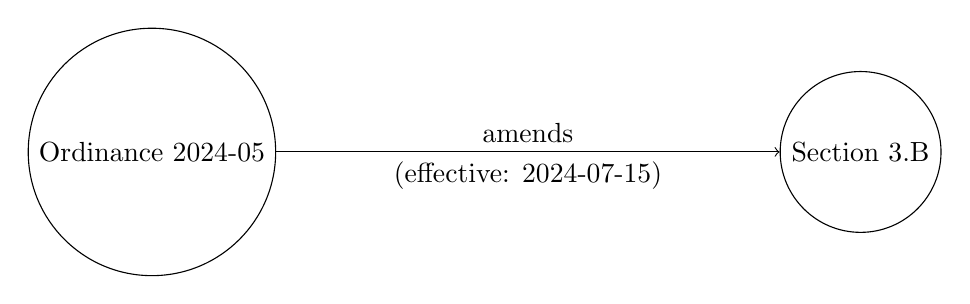
\begin{tikzpicture}[node distance={90mm}, main/.style = {draw, circle}]
 \node[main] (1) {Ordinance 2024-05};
 \node[main] (2) [right of=1] {Section 3.B};
 \draw[->] (1) -- node[midway, above] {amends} node[midway, below] {(effective: 2024-07-15)} (2);
\end{tikzpicture}
\captionsetup{
    labelfont={bf,it}, 
    textfont=it,  
    justification=centering
    }
\caption{Knowledge graph fragment of a legal amendment.}
\label{fig:simple_kg}
\end{figure}

Pioneering work in structured knowledge includes Minsky's concept of Frames\index{Minsky, Marvin}\index{Knowledge Graphs!frames}, which represented stereotypical situations using slots and relationships, thereby influencing subsequent formalisms like description logics and semantic web ontologies \parencite{RefWorks:RefID:78-minsky1974framework}.

\subsection{The Role of Ontologies and Schema in KG Construction}
\label{subsec:ontologies}
A Knowledge Graph's utility for analytical tasks extends beyond its raw structure of nodes and edges; it is deeply rooted in the formal schema, or ontology, that governs it. An ontology serves as the conceptual blueprint for the knowledge domain, explicitly defining the types of entities (classes), their attributes (properties), and the permissible relationships between them \parencite{RefWorks:RefID:135-noy2001ontology}. In the context of legal documents, an ontology might define classes such as \texttt{Ordinance}, \texttt{DefinedTerm}, and \texttt{ZoningDistrict}, along with rules specifying that an \texttt{Ordinance} can have an \texttt{enactmentDate} property of type \texttt{Date} and can be linked to a \texttt{DocumentSection} via an \texttt{AMENDS} relationship.

This formal specification is not merely a descriptive convenience; it is a prerequisite for automated validation. By defining a clear schema, one can programmatically check for both consistency and completeness. Consistency is checked by identifying graph structures that violate the ontological rules. For example, if a node representing a township is linked to a \texttt{PermittedUse} node, this would violate a schema rule stating that only \texttt{ZoningDistrict} nodes can have such a relationship. Completeness can be assessed against schema-defined cardinality constraints. If the ontology specifies that every \texttt{DefinedTerm} node \textit{must} have at least one incoming \texttt{DEFINES} relationship from a \texttt{DocumentSection} node, any such node lacking this relationship represents an instance of structural incompleteness within the KG, signaling a potential flaw in the source document. Thus, the ontology transforms the KG from a simple data structure into a formal model against which the document's integrity can be rigorously tested.

\subsection{Reasoning Over Knowledge Graphs}
\label{subsec:kg_reasoning}
The true analytical power of a Knowledge Graph is unlocked through reasoning—the process of inferring implicit knowledge from the explicitly asserted facts. Reasoning enables the discovery of relationships and properties that are not directly stated in the source text, allowing for a deeper and more comprehensive analysis. Two primary modes of reasoning are relevant to document validation: deductive and inductive.

Deductive reasoning uses a set of logical rules and axioms, often defined in the ontology, to derive new conclusions with certainty. Technologies like the Web Ontology Language (OWL) and the Shapes Constraint Language (SHACL) provide formalisms for expressing these rules \parencite{RefWorks:RefID:110-hitzler2009foundations, RefWorks:RefID:154-knublauch2017shapes}. For example, if the KG contains the facts (\texttt{Ordinance\_123}, \texttt{AMENDS}, \texttt{Section\_3.B}) and (\texttt{Section\_3.B}, \texttt{PART\_OF}, \texttt{Article\_III}), a deductive reasoner could apply a transitivity rule to infer the new triple (\texttt{Ordinance\_123}, \texttt{IMPACTS}, \texttt{Article\_III}). This capability is crucial for identifying the far-reaching consequences of amendments and for detecting logical contradictions that may only become apparent through multi-step inference.

Inductive reasoning, in contrast, is probabilistic and is typically performed using machine learning models that operate on graph structures, such as Graph Neural Networks (GNNs) \parencite{RefWorks:RefID:7-gupta2021graph}. A primary application of inductive reasoning in KGs is link prediction, where the model learns patterns from the existing graph structure to predict the likelihood of missing edges between nodes. In the context of document analysis, link prediction could identify a likely but absent \texttt{USES\_TERM} relationship between a section of text and a relevant defined term, flagging a potential omission for human review. While not logically certain, this inductive approach provides a powerful tool for identifying gaps and enhancing the completeness of the knowledge base.

\subsection{KG Technologies and Applications}
\label{subsec:kg_techandapp}

Knowledge graphs are implemented using various technologies. The Resource Description Framework (RDF)\index{Knowledge Graphs!RDF} is a W3C standard based on triples (subject-predicate-object) and is foundational to the Semantic Web\index{Semantic Web}. It is often queried using SPARQL\index{SPARQL} and defined with ontology languages like OWL\index{Ontology!OWL} \parencite{RefWorks:RefID:109-2025rdf, RefWorks:RefID:111-kumar2013querying, RefWorks:RefID:110-hitzler2009foundations}. Property Graphs\index{Knowledge Graphs!Property Graphs}, used in databases like Neo4j, offer a flexible model where both nodes and edges can have properties and are queried with languages like Cypher or Gremlin \parencite{RefWorks:RefID:114-fernandes2018graph}. Additionally, Graph Neural Networks (GNNs)\index{Graph Neural Networks (GNNs)} are machine learning techniques that operate on graph structures to learn vector representations (embeddings\index{Embeddings}), enabling tasks like link prediction and node classification \parencite{RefWorks:RefID:7-gupta2021graph, RefWorks:RefID:47-scarselli2009graph, RefWorks:RefID:49-wang2024graph}.

KGs are employed in diverse applications, including semantic search, recommendation systems, and enterprise data integration \parencite{RefWorks:RefID:102-hogan2021knowledge, RefWorks:RefID:118-ji2022survey, RefWorks:RefID:120-fensel2020knowledge}. Their ability to explicitly model complex relationships makes them valuable for analyzing the internal structure and integrity of large document collections.

\section{Information Extraction for KG Construction}
To leverage KGs for document analysis, the unstructured information within source documents must be transformed into the structured format of a graph. This process, termed KG construction\index{Knowledge Graphs!construction}, relies on Information Extraction (IE)\index{Information Extraction (IE)} techniques \parencite{RefWorks:RefID:121-zhong2024comprehensive, RefWorks:RefID:122-kolluru2020imojie}. This section covers two fundamental IE tasks: identifying nodes via Named Entity Recognition (NER)\index{Named Entity Recognition (NER)} and identifying edges via Relation Extraction (RE)\index{Relation Extraction (RE)}. LLMs have shown significant promise in performing both tasks, often with minimal task-specific training data \parencite{RefWorks:RefID:107-benjira2025automated}.

\subsection{Named Entity Recognition}
Named Entity Recognition (NER) is a primary task in information extraction that identifies and classifies named entities in text into predefined categories \parencite{RefWorks:RefID:4-al-moslmi2020named}. These categories can include standard types like persons and organizations or be extended to domain-specific entities. For building KGs, NER serves as the main mechanism for identifying the potential \textbf{nodes} of the graph. A subsequent step, Entity Linking\index{Entity Linking}, is often necessary to disambiguate these mentions and link them to unique identifiers \parencite{RefWorks:RefID:5-chaurasiya2022entity}.

NER methods have evolved significantly. Early approaches were rule-based systems\index{Named Entity Recognition (NER)!rule-based} that used hand-crafted rules and dictionaries, which achieved high precision but were brittle and labor-intensive \parencite{RefWorks:RefID:126-nadeau2007survey, RefWorks:RefID:127-grishman1996messageunderstanding}. These were followed by statistical models\index{Named Entity Recognition (NER)!statistical models} like Hidden Markov Models and Conditional Random Fields, which offered better generalization \parencite{RefWorks:RefID:128-lafferty2001conditional}. Currently, deep learning approaches\index{Named Entity Recognition (NER)!deep learning}, particularly Transformer-based models like BERT, have achieved state-of-the-art performance by leveraging powerful pre-trained representations \parencite{RefWorks:RefID:4-al-moslmi2020named, RefWorks:RefID:57-carbonell2020named}.

Applying NER to the legal domain requires identifying specialized entities such as specific statutes, defined legal terms, legal roles, and explicit document references \parencite{RefWorks:RefID:124-au2022ener, RefWorks:RefID:125-kalamkar2022named}. The unique vocabulary and complex sentence structures of legal texts necessitate that NER models be trained or fine-tuned on legally annotated corpora to achieve high accuracy \parencite{RefWorks:RefID:64-2022lexglue}. A robust legal NER system provides the essential building blocks for constructing a meaningful knowledge graph from legal documents.

\subsection{Relation Extraction}
While NER identifies entities (nodes), Relation Extraction (RE)\index{Relation Extraction (RE)} identifies the semantic relationships between them, which correspond to the edges in a knowledge graph \parencite{RefWorks:RefID:118-ji2022survey, RefWorks:RefID:57-carbonell2020named}. For instance, from the sentence "Acme Corp, headquartered in West Chester, acquired Beta Inc.," RE aims to identify relations such as `headquarteredIn(Acme Corp, West Chester)`. This task is crucial for building the graph's structure. Work in this area includes both Closed RE, for a predefined set of relation types, and Open Information Extraction (OpenIE)\index{Information Extraction (IE)!OpenIE}, which extracts relations expressed with arbitrary text \parencite{RefWorks:RefID:134-etzioni2008acm}.

Approaches to RE have mirrored those in NER. Early systems were rule-based\index{Relation Extraction (RE)!rule-based}, using linguistic patterns to identify relations \parencite{RefWorks:RefID:136-hearst1992automatic}. Supervised statistical models\index{Relation Extraction (RE)!statistical models} followed, using classifiers trained on annotated data or data generated through distant supervision\index{Relation Extraction (RE)!distant supervision}, a technique that aligns known relations from KGs with text but can introduce noise \parencite{RefWorks:RefID:139-kambhatla2004combining, RefWorks:RefID:140-mintz2009distant}. Modern deep learning approaches\index{Relation Extraction (RE)!deep learning}, especially Transformer-based models, now represent the state-of-the-art \parencite{RefWorks:RefID:141-kumar2017survey, RefWorks:RefID:142-wu2019enriching}. LLMs, through prompting techniques, offer a powerful alternative capable of extracting relations with minimal task-specific fine-tuning \parencite{RefWorks:RefID:143-chia2022relation}.

Key challenges in RE include handling ambiguity, extracting relations that span sentences, and adapting models to new domains. In the legal context, extracting relations such as amendments, definitions, and obligations is critical for building a KG that accurately reflects the legal framework \parencite{RefWorks:RefID:77-tauqeer2022automated, RefWorks:RefID:76-dhani2021similar}. The structured output from NER and RE forms the basis for the constructed knowledge graph.

\section{Consistency, Completeness, and Coherence}
When analyzing formal document corpora such as legal codes or technical standards, quality evaluation often involves assessing internal integrity. Three key aspects of this integrity are consistency\index{Consistency}, completeness\index{Completeness}, and coherence\index{Coherence} \parencite{RefWorks:RefID:29-umar2024advances}. These concepts, while sometimes overlapping, address distinct facets crucial for ensuring documents are understandable, unambiguous, and effective.

\begin{itemize}
    \item \textbf{Consistency:}\index{Consistency} Refers to the absence of logical contradictions within a document set \parencite{RefWorks:RefID:10-zowghi2003interplay, RefWorks:RefID:21-heitmeyer1996automated, RefWorks:RefID:25-nentwich2005managing, RefWorks:RefID:26-egyed2006instant, RefWorks:RefID:27-tröls2022instant, RefWorks:RefID:28-yang2024fizz, RefWorks:RefID:30-guo2023joint}. A consistent document should not contain provisions that assert mutually exclusive facts or prescribe conflicting obligations under identical conditions. Detecting such inconsistencies is vital for legal certainty and predictability \parencite{RefWorks:RefID:52-donelson2019legal, RefWorks:RefID:53-duck-mayr2022explaining, RefWorks:RefID:54-rossi2016inconsistent}. Formal logic and automated reasoning techniques are often employed to check consistency in formal specifications \parencite{RefWorks:RefID:21-heitmeyer1996automated, RefWorks:RefID:24-brucker2019ontologies}.

    \item \textbf{Completeness:}\index{Completeness} Pertains to whether the document set contains all necessary information relative to its intended scope \parencite{RefWorks:RefID:10-zowghi2003interplay}. Defining completeness is inherently challenging, as it depends on a clear specification of what should be included. In a legal context, completeness may require that all terms are adequately defined, referenced procedures are specified, and relevant scenarios are addressed. Gaps or omissions can lead to ambiguity and disputes. Assessing completeness often requires significant domain knowledge and may involve checking against predefined templates or requirements specifications \parencite{RefWorks:RefID:10-zowghi2003interplay, RefWorks:RefID:29-umar2024advances}. The interpretation of completeness in KGs is also affected by the "Closed World Assumption" versus the "Open World Assumption"\index{Knowledge Graphs!reasoning!Closed World Assumption} \parencite{RefWorks:RefID:148-reiter1978on, RefWorks:RefID:110-hitzler2009foundations}.

    \item \textbf{Coherence:}\index{Coherence} Relates to the overall understandability, organization, and logical flow of the presented information \parencite{RefWorks:RefID:44-wang2014short, RefWorks:RefID:14-shen2021evaluating}. A coherent document is well-structured, uses terminology consistently, and ensures cross-references are accurate. While related to consistency, coherence focuses more on clarity and comprehensibility for a human reader, encompassing aspects like lexical cohesion and discourse structure \parencite{RefWorks:RefID:44-wang2014short}.
\end{itemize}

Ensuring these three qualities simultaneously in large, evolving legal codes through traditional manual review is exceptionally difficult. The volume of text, the intricate web of interdependencies, the potential for ambiguity in natural language, and the distributed nature of authorship make manual detection of subtle flaws challenging and error-prone \parencite{RefWorks:RefID:68-beth2018bills}. Computational approaches that leverage structured representations like KGs offer significant potential advantages.

A Knowledge Graph provides a structured substrate amenable to automated analysis by explicitly modeling entities and their relationships. Graph-based queries and algorithms can be designed to automatically detect potential inconsistencies, such as conflicting property values or circular definition chains \parencite{RefWorks:RefID:77-tauqeer2022automated, RefWorks:RefID:24-brucker2019ontologies, RefWorks:RefID:19-schönberg2011verifying, RefWorks:RefID:23-weitl2006checking}. While perfect completeness verification is often intractable for natural language documents, KGs can help identify potential gaps by analyzing the graph's structure for missing nodes, absent relationships, or orphaned sections \parencite{RefWorks:RefID:151-rabbani2023extraction, RefWorks:RefID:152-rabbani2022shacl, RefWorks:RefID:153-omran2020shacl, RefWorks:RefID:154-knublauch2017shapes, RefWorks:RefID:29-umar2024advances}.

LLMs can play a role throughout this pipeline, aiding in the initial interpretation of text to populate the KG, helping to formulate complex graph queries, or summarizing the findings from the analysis for human review \parencite{RefWorks:RefID:107-benjira2025automated}. The KG itself, however, provides the persistent, globally coherent, and computationally tractable structure necessary for systematic integrity checks. Such a structure can overcome the context window limitations and potential lack of deterministic reasoning inherent in LLMs alone. Research exploring KGs and related AI techniques for automated integrity checking provides a foundation for this approach \parencite{RefWorks:RefID:29-umar2024advances, RefWorks:RefID:21-heitmeyer1996automated, RefWorks:RefID:77-tauqeer2022automated, RefWorks:RefID:76-dhani2021similar, RefWorks:RefID:11-aumiller2021structural}. This praxis project aims to build upon such work by investigating the practical application of LLM-driven KG construction for analyzing municipal legal codes.

\section{Challenges in Analyzing Large Documents} \label{sec:doc_processing}
Research in automated document processing is extensive, covering tasks like summarization, information extraction, and question answering \parencite{RefWorks:RefID:156-gambhir2017recent, RefWorks:RefID:121-zhong2024comprehensive, RefWorks:RefID:157-2017reading}. Historically, much of this research focused on relatively small documents, as they are less computationally demanding and more feasible for the human evaluation required to establish ground truth.

Many critical real-world applications, however, involve documents that are orders of magnitude larger, such as legal contracts, technical manuals, and extensive regulatory codes. Analyzing these large documents\index{Document Processing!large documents} presents distinct and significant challenges:
\begin{itemize}
    \item \textbf{Computational Resources:}\index{Document Processing!large documents!computational resources} Processing large volumes of text demands substantial memory, storage, and processing time. The computational complexity often scales non-linearly with document length, making naive processing of entire large documents infeasible \parencite{RefWorks:RefID:81-vaswani2017attention}.
    \item \textbf{Long-Range Dependencies:}\index{Document Processing!large documents!long-range dependencies} Comprehension frequently requires capturing semantic connections or references between sections that are far apart in the document. Models with limited context windows struggle to capture these long-distance relationships accurately \parencite{RefWorks:RefID:99-liu2025comprehensive, RefWorks:RefID:101-zhao2023survey}.
    \item \textbf{Context Fragmentation:}\index{Document Processing!large documents!context fragmentation} A common technique for handling large documents involves splitting them into smaller chunks. This method, while necessary for models with fixed inputs, risks losing critical context that spans chunk boundaries, potentially leading to fragmented understanding \parencite{RefWorks:RefID:105-chen2024dense, RefWorks:RefID:104-qu2024semantic}.
    \item \textbf{Evaluation Complexity:}\index{Document Processing!large documents!evaluation complexity} Assessing the quality of automated analysis on a large document is inherently difficult for human evaluators. Establishing reliable ground truth for evaluation benchmarks remains a major challenge for large-document tasks \parencite{RefWorks:RefID:116-shaham2022scrolls}.
\end{itemize}
Techniques like Retrieval-Augmented Generation (RAG)\index{Retrieval-Augmented Generation (RAG)} allow LLMs to leverage information from large external corpora without processing the entire corpus in their context window \parencite{RefWorks:RefID:158-lewis2020retrievalaugmented}. RAG retrieves relevant text snippets and provides them as context to the LLM. Although powerful for knowledge-intensive tasks, standard RAG retrieves discrete, localized chunks and may not provide the holistic, structured view of the entire document that a pre-constructed Knowledge Graph can offer.

\section{Challenges in Analyzing Legal Documents} \label{sec:legal_docs}
Legal documents, particularly statutory codes, represent a compelling yet challenging domain for advanced document analysis techniques. They possess several intrinsic characteristics that make them difficult testbeds and valuable targets for automation:\index{Legal Document Analysis}
\begin{itemize}
    \item \textbf{Complexity and Precision:}\index{Legal Document Analysis!complexity and precision} Legal language is dense, employing specialized terminology and complex sentence structures. Ambiguity must be minimized, demanding high precision in interpretation, as misinterpretations can have significant real-world consequences \parencite{RefWorks:RefID:159-ashley2017artificial, RefWorks:RefID:62-malik2022semantic}.
    \item \textbf{Volume and Interconnectedness:}\index{Legal Document Analysis!volume and interconnectedness} Legal corpora can be vast and are highly interconnected through citations, amendments, and definitions. Understanding one part often requires understanding its relationship to many others \parencite{RefWorks:RefID:68-beth2018bills}.
    \item \textbf{Semi-structured Format:}\index{Legal Document Analysis!semi-structured format} Legal texts mix structured elements (e.g., sections, clauses) with unstructured natural language prose, requiring sophisticated NLP techniques to handle both.
    \item \textbf{Critical Need for Integrity:}\index{Legal Document Analysis!integrity} The consistency, completeness, and coherence of legal documents are paramount for their function. These qualities underpin the rule of law, ensuring predictability and enforceability. Flaws can lead to disputes, costly litigation, and erosion of public trust \parencite{RefWorks:RefID:52-donelson2019legal, RefWorks:RefID:53-duck-mayr2022explaining, RefWorks:RefID:54-rossi2016inconsistent}.
\end{itemize}

The specific focus on the codified ordinances of Pennsylvania townships provides a valuable and concrete dataset. These codes exhibit realistic complexity, having often been developed over decades with multiple authorships and numerous amendments. The legislative drafting and codification process, although designed to ensure quality through multi-stage human review, can still introduce errors. Inconsistencies, incompleteness, and incoherence can persist as the code grows \parencite{RefWorks:RefID:54-rossi2016inconsistent}. The resource-intensive and fallible nature of purely manual review motivates the exploration of computational methods to assist legal professionals in maintaining the integrity of these foundational legal documents.

\section{Related Work} % Needs to be filled with actual citations
Research relevant to this praxis project spans several areas: utilizing LLMs for Information Extraction, applying KGs for document integrity checking, and the application of NLP to the legal domain.

\textbf{LLMs for Information Extraction and KG Construction:}\index{Information Extraction (IE)!using LLMs}\index{Knowledge Graphs!construction!using LLMs}
The advent of powerful LLMs has advanced information extraction. Studies demonstrate the ability of models like GPT-4, often via prompting, to perform NER and RE with performance rivaling or exceeding traditional fine-tuned models, especially in specialized domains \parencite{RefWorks:RefID:160-xu2024large}. Researchers have explored various techniques to mitigate LLM limitations like hallucinations\index{Large Language Models (LLMs)!hallucinations} and to control output structure \parencite{RefWorks:RefID:87-wang2023gptner}. Several works focus on constructing KGs from text using LLMs as the primary extraction engine, developing pipelines that integrate entity identification, relation extraction, and schema mapping, sometimes with human-in-the-loop refinement \parencite{RefWorks:RefID:107-benjira2025automated, RefWorks:RefID:162-lairgi2024knowledge}.

\textbf{KGs for Document Analysis and Integrity Checking:}\index{Knowledge Graphs!for document analysis}
Beyond construction, KGs serve as a substrate for advanced document analysis, including semantic search and complex question answering \parencite{RefWorks:RefID:102-hogan2021knowledge, RefWorks:RefID:118-ji2022survey}. Directly relevant to this work is the use of KGs for consistency and completeness checking. In software requirements engineering, KGs and ontologies model requirements to detect conflicts \parencite{RefWorks:RefID:29-umar2024advances}. In the Semantic Web community, technologies like SHACL (Shapes Constraint Language)\index{SHACL (Shapes Constraint Language)} provide a standard way to validate RDF KGs against predefined constraints, effectively checking aspects of data integrity \parencite{RefWorks:RefID:154-knublauch2017shapes}.

\textbf{AI and NLP for Legal Document Analysis:}\index{Legal Document Analysis}
The legal domain has been a target for AI and NLP research for decades \parencite{RefWorks:RefID:159-ashley2017artificial}. Recent research applies modern NLP to tasks like legal information retrieval, case outcome prediction, and contract review \parencite{RefWorks:RefID:45-moens2001innovative, RefWorks:RefID:164-aletras2016predicting, RefWorks:RefID:64-2022lexglue}. Information extraction from legal texts has received significant attention, focusing on extracting citations, legal entities, and obligations \parencite{RefWorks:RefID:125-kalamkar2022named, RefWorks:RefID:77-tauqeer2022automated}. Some prior work has explored automated consistency checking in legal documents, often using rule-based or logic-based approaches, but these efforts have typically focused on specific types of conflicts rather than a comprehensive KG-based approach applied to municipal codes \parencite{RefWorks:RefID:54-rossi2016inconsistent}.

\subsection{Unique Linguistic Features of Legal Text}
\label{subsec:legal_linguistics}
The analysis of legal documents constitutes a distinct and challenging subfield of NLP, often referred to as Legal AI, due to the unique linguistic register, or "legalese," employed in these texts \parencite{RefWorks:RefID:159-ashley2017artificial}. This register presents formidable obstacles for standard NLP models that are typically trained on general-domain corpora. Key features include:

\begin{itemize}
    \item \textbf{Deontic Modality:} Legal texts are saturated with the language of obligations, permissions, and prohibitions, expressed through modal verbs such as \textit{shall}, \textit{must}, \textit{may}, and \textit{is prohibited} \parencite{RefWorks:RefID:186-navarro2014deontic}. Accurately parsing these expressions to extract the agent (who is obligated), the action (what must be done), and the specific modal force is essential for modeling the regulatory framework encoded in the text.
    \item \textbf{Intertextuality:} Legal documents rarely exist in isolation. Their meaning is constructed through a dense web of internal and external citations, such as ``as defined in Section 3.B'' or ``pursuant to 53 Pa.C.S.A. § 101''. This high degree of intertextuality means that a document's semantic content is distributed across multiple locations, making the modeling of these referential links—an inherently graph-like problem—paramount for any coherent analysis.
    \item \textbf{Controlled Vocabulary and Ambiguity:} While legal language strives for precision through a controlled vocabulary of defined terms, it is also rife with potential ambiguity. Syntactic ambiguity can arise from complex sentence structures with long, nested clauses, making it difficult to determine the scope of modifiers (the "dangling else" problem). Semantic ambiguity can occur when a term has a specific legal meaning that differs from its common usage.
\end{itemize}
These unique challenges necessitate specialized NLP approaches that can move beyond simple entity recognition to a more nuanced extraction of structured legal rules, definitions, and deontic relationships.

\subsection{A Brief History of Computational Law}
\label{subsec:legal_ai_history}
The application of computational methods to legal text is not a new endeavor; the field of Computational Law has evolved over several decades, mirroring broader trends in artificial intelligence. Understanding this history provides context for the contemporary approaches leveraged in this praxis.

The earliest forays into Legal AI, beginning in the 1970s and 1980s, were dominated by rule-based expert systems \parencite{RefWorks:RefID:187-susskind1986expert}. These systems attempted to capture legal knowledge by having human experts manually encode statutes and case law into formal logic, often using languages like Prolog. While pioneering, these systems were brittle, struggled to handle legal ambiguity, and faced an insurmountable "knowledge acquisition bottleneck," as the manual encoding process was extraordinarily labor-intensive.

The subsequent era saw a shift toward statistical methods and the rise of large-scale legal databases like Westlaw and LexisNexis. The primary focus of NLP during this period was on Legal Information Retrieval (LIR), using techniques from information retrieval to improve the search and discovery of relevant documents for legal professionals. This period also saw the application of machine learning to tasks such as e-discovery, where algorithms were used to classify documents as relevant or non-relevant to a case, drastically reducing the burden of manual review.

The modern era of Computational Law is defined by the advent of deep learning and, most recently, Large Language Models. Transformer-based models have achieved state-of-the-art results on a variety of legal tasks, including predicting judicial decisions from case texts \parencite{RefWorks:RefID:164-aletras2016predicting}, automated summarization of legal opinions, and the analysis and clause extraction from contracts. The research presented in this praxis is situated within this modern paradigm, applying the powerful generative and analytical capabilities of LLMs to the foundational but often-overlooked task of ensuring the internal structural integrity of the legislative documents that form the basis of the rule of law.

\textbf{Positioning of this Work:}
This praxis project builds upon these converging lines of research. While previous work has explored LLMs for KG construction and KGs for consistency checking separately, the specific contribution here lies in the integration and practical application of modern LLMs to construct KGs from municipal legal codes for consistency and completeness analysis. The project addresses LLM context window limitations by leveraging the KG structure for global reasoning. Unlike prior legal AI work focusing on case law or contracts, this project targets foundational legislative texts at the local government level. The "praxis" aspect emphasizes developing and evaluating a practical methodology to assist municipal professionals in maintaining the quality of their codified laws.

\section{Conclusions}

This review of the literature establishes a foundational tension in modern NLP: while Large Language Models built on the Transformer architecture possess unprecedented text processing capabilities, their inherent context window limitations prevent the holistic analysis required for verifying the integrity of large documents \parencite{RefWorks:RefID:81-vaswani2017attention, RefWorks:RefID:99-liu2025comprehensive}. The research surveyed demonstrates that Knowledge Graphs (KGs) present a robust solution to this challenge by transforming unstructured text into a persistent, structured, and globally queryable representation of knowledge \parencite{RefWorks:RefID:102-hogan2021knowledge}.

The process of Information Extraction, encompassing Named Entity Recognition (NER) and Relation Extraction (RE), serves as the critical bridge between the unstructured document and the structured KG \parencite{RefWorks:RefID:160-xu2024large}. By leveraging a KG, the core quality attributes of a document—\textbf{consistency}, \textbf{completeness}, and \textbf{coherence}—are made computationally tractable. This allows for systematic analysis that can overcome the limitations of manual review, which is particularly error-prone in dense, interconnected legal corpora \parencite{RefWorks:RefID:10-zowghi2003interplay, RefWorks:RefID:68-beth2018bills}.

While the literature addresses LLM-driven knowledge extraction, KG-based analysis, and Legal AI as separate fields, this project is situated at their practical synthesis. The novel contribution of this work is the integration of these techniques into a single framework focused specifically on analyzing the structural integrity of municipal legal codes. The limitations of current models and the critical need for reliable legal frameworks, as established in this review, directly motivate the methodology of this praxis project. The following chapter will detail the specific methodology employed to construct and evaluate a system designed to achieve this objective.
